\documentclass[conference]{IEEEtran}
\IEEEoverridecommandlockouts
% The preceding line is only needed to identify funding in the first footnote. If that is unneeded, please comment it out.
\usepackage{cite}
\usepackage{amsmath,amssymb,amsfonts}
\usepackage{algorithmic}
\usepackage{graphicx}
\usepackage{textcomp}
\usepackage{xcolor}

\usepackage{tabularx}
\usepackage{booktabs}
\usepackage{array}
\usepackage{xurl}
\usepackage{tikz}
\usetikzlibrary{arrows.meta,positioning,shapes.geometric,fit,backgrounds}

\def\BibTeX{{\rm B\kern-.05em{\sc i\kern-.025em b}\kern-.08em
    T\kern-.1667em\lower.7ex\hbox{E}\kern-.125emX}}
\begin{document}

\title{SafeStream-Kafka: Real-Time Safety Analytics for IoT Workplace Video Streams\textsuperscript{*}\\
\thanks{\textsuperscript{*}~The complete source code is available at \protect\url{https://github.com/Lumysia/SafeKafka}.}
}

\author{
\IEEEauthorblockN{
Vitor Brandao Raposo,
Yujie Lin,
Livia Zhang,
Quang Thong Phung,
and Ahmed Seyam
}
\IEEEauthorblockA{
Faculty of Engineering and Applied Science\\
Ontario Tech University\\
Oshawa, Ontario, Canada
}
}

\maketitle
% =========================================================
% abstract
% =========================================================
\begin{abstract}
SafeStream-Kafka is a prototype for real time safety analytics on IoT style workplace video streams. It uses Apache Kafka to move frame events between services, OpenCV to extract and encode frames, an Ultralytics YOLO per frame classifier (the code also supports a detection mode) to label safety related behavior, a rolling-window aggregator to calculate per camera metrics, and a FastAPI dashboard for live monitoring. The pipeline accepts CCTV, RTSP, webcam, or replayed video sources; labels each processed frame as safe, unsafe, or other; tracks cumulative and rolling unsafe ratios; and publishes alerts when unsafe activity crosses a threshold. Across six models compared on this dataset, the classifier had the highest offline accuracy and produced the fewest false alerts in the stream. On the live pipeline, we additionally measure system behavior, including a mean end to end latency of approximately 0.2 s through a cloud broker, throughput that tracks the input rate with zero consumer lag, and the network cost of transporting base64-encoded JPEG frames, throughput that tracks the input rate with zero consumer lag, and the network cost of moving base64 encoded JPEG frames. The report documents the motivation, background, architecture, methodology, evaluation results, limitations, and remaining work.
\end{abstract}

\begin{IEEEkeywords}
Apache Kafka, IoT video analytics, YOLO, workplace safety,
real-time stream processing, FastAPI
\end{IEEEkeywords}


% =========================================================
% 1. Problem Definition and Motivation
% =========================================================
\section{Problem Definition and Motivation}
Unsafe behavior in workplaces puts workers, equipment, and production schedules at immediate risk. Industrial and construction sites already run CCTV or network cameras, but raw video is hard to monitor continuously by hand. The analytics problem is to turn those streams into timely safety signals: unsafe-behavior counts, rolling violation ratios, and high-severity alerts that a supervisor can act on.

SafeStream-Kafka treats this video as an IoT data stream rather than an offline video-processing task. It ingests live or realistically replayed video, classifies safety related behavior frame by frame, aggregates the results per camera, and surfaces live operational metrics in a web dashboard. The scope fits the graduate real-time analytics rubric: it handles streaming data, applies machine learning inference, delivers a working prototype, and exposes measurable quantities such as alert rates, rolling ratios, and processing throughput.

We also study the classifier itself as a real time alert source. Prior work on safety behavior recognition reports \emph{offline} accuracy (measured on a fixed, pre recorded test set rather than on the live stream); we instead run the model as a Kafka \emph{stream} and measure its \emph{streaming} behavior on the running pipeline, as alerts are produced. While the gap between offline and online performance and the need for per-model decision thresholds are familiar in machine learning generally, we are not aware of prior work that measures them for this safety behavior task on a running stream processing pipeline. We find that offline accuracy does not by itself rank models by their streaming false alert behavior, that the alert level must be set per model, and that a per frame classifier matches or exceeds temporal \emph{window models} (which classify a short stack of consecutive frames rather than one frame) on accuracy and alert quality at lower per frame cost.

The project objectives are:

\begin{itemize}
\item Ingest video from files, directories, RTSP streams, or webcams and publish frames as Kafka events.
\item Run YOLO classifier on each frame to label safety behavior (a detection mode is also available in code).
\item Convert model labels into safe, unsafe, or other categories.
\item Maintain per camera cumulative counts, rolling-window unsafe ratios, violation labels, and alert history.
\item Serve a live dashboard with camera cards, current frame snapshots, recent alerts, and violation frame endpoints.
\item Provide reproducible scripts for topic creation, dataset preparation, model training, and local or cloud Kafka deployment.
\end{itemize}

\subsection{Research Questions}
\label{subsec:research-questions}

Beyond building the prototype, the project sets out to answer three
research questions about running a safety classifier as a real time alert
source. These questions are stated here and answered with measured results
in Section~\ref{subsec:findings}.

\begin{itemize}
\item \textbf{RQ1.} Does a model's \emph{offline} classification accuracy
predict its \emph{streaming} false alert behavior, or must the two be
measured separately?

\item \textbf{RQ2.} Do temporal window models outperform a single-frame
classifier on accuracy and alert quality for safety behaviors that are
visible in one frame, and is the extra per frame cost justified?

\item \textbf{RQ3.} Can one fixed alert threshold serve every model, or
must the alert level be \emph{calibrated} per model choosing its trigger
level on a validation set because each puts its unsafe probability on a
different scale?
\end{itemize}

% =========================================================
% 2. Literature Review and Background
% =========================================================
\section{Literature Review and Background}

\subsection{Streaming Video Analytics for IoT}

Streaming video analytics has a simple requirement and a difficult systems constraint: frames arrive continuously, but the model, broker, dashboard, and alert logic do not all run at the same pace. Edge and IoT video analytics surveys point to the same pressure points: high data volume, latency sensitivity, and expensive deep learning inference~\cite{b1,b2}. SafeStream-Kafka handles those constraints by separating ingestion, inference, aggregation, and visualization instead of forcing every stage through one process.

That separation is what makes the project a streaming analytics prototype rather than a single offline computer vision script.

\subsection{Apache Kafka as a Streaming Backbone}

Kafka was designed to move high volume event data with low latency~\cite{b3}. In SafeStream-Kafka, each stage reads and writes a topic without sharing memory or process state. The topic boundaries are explicit: cctv-frames carries encoded video frames, safety detections carries model outputs, and safety alerts carries aggregated alert events.

The implementation can point either to Confluent Cloud or to a local plaintext broker. The producer enables compression, idempotent delivery, and larger message limits because JPEG frame payloads are much larger than ordinary log lines. Consumers use separate group IDs, so the dashboard, detector, and aggregator can process the same topics without sharing offset state.

\subsection{YOLO for Real-Time Visual Analytics}
Ultralytics YOLO supports two related tasks: detection, which needs bounding boxes, and classification, which assigns one label to a whole frame~\cite{b4,b5}. That distinction matters for this dataset. The selected safety-behavior clips~\cite{b6} are labeled at the clip level, not with bounding boxes, so this project uses the classification task; the code keeps a detection mode for a later bounding-box dataset.

The detector does not treat YOLO output as the final product. It turns raw labels into normalized safe, unsafe, or other categories, then publishes a compact JSON summary with camera ID, frame ID, source, timestamp, detections, safe count, unsafe count, and total detections.

\subsection{Video Action-Recognition Models}
\label{subsec:action-models}

The per frame classifier above labels each frame independently, while temporal
window models classify short stacks of consecutive frames to test whether motion
improves safety recognition. We compare the per-frame YOLO classifier with five
temporal-window baselines: ResNet18+GRU, R(2+1)D-18, MViTv2-S, Video Swin-T, and
Hiera-B. The transformer models were pretrained on Kinetics-400 and linear-probed
to fit the available 8\,GB GPU budget.

% The per-frame classifier above labels each frame independently, but many
% unsafe behaviors play out over time. A second model family---temporal
% window models---instead classifies a short stack of consecutive frames,
% trading per-frame cost for access to motion cues. To test whether that
% extra modeling helps on this dataset (Section~\ref{subsec:research-questions},
% RQ2), the comparison in Section~\ref{subsec:findings} places the per-frame
% YOLO classifier against five window models drawn from the
% action-recognition literature.

% \begin{itemize}
%     \item \textbf{Per-frame YOLO classifier} labels each frame on its own
%     and serves as the single-frame point of comparison; it carries no
%     cross-frame temporal information.

%     \item \textbf{ResNet18 + GRU head} is the simple in-house baseline: a
%     two-dimensional convolutional ResNet~\cite{b11} extracts per-frame
%     features that a gated recurrent unit (GRU)~\cite{b12} reads in sequence
%     across the window. It is included as a lightweight baseline rather than
%     a state-of-the-art model.

%     \item \textbf{R(2+1)D-18} factorizes each three-dimensional convolution
%     into a separate spatial convolution followed by a separate temporal
%     convolution, which improves action recognition while keeping the
%     parameter count modest~\cite{b7}.

%     \item \textbf{MViTv2-S} is a multiscale vision transformer that builds a
%     feature pyramid inside the transformer, progressively trading spatial
%     resolution for channel depth for efficient video classification~\cite{b8}.

%     \item \textbf{Video Swin-T} is a video transformer that restricts
%     self-attention to local, shifted three-dimensional windows, giving a
%     strong accuracy--efficiency trade-off for video~\cite{b9}.

%     \item \textbf{Hiera-B} is a hierarchical vision transformer that drops
%     the specialized modules added by earlier hierarchical models and instead
%     learns spatial structure through masked-autoencoder pretraining~\cite{b10}.
% \end{itemize}

% The three transformers (MViTv2-S, Video Swin-T, and Hiera-B) are pretrained
% on the Kinetics-400 action-recognition dataset~\cite{b13} and are used here
% as strong action-recognition baselines. Rather than fine-tuning their large
% backbones, this project \emph{linear-probes} them---training only a new final
% layer on top of the frozen pretrained network---so that the comparison stays
% within a single 8\,GB GPU.


% =========================================================
% 3. System Design and Methodology
% =========================================================
\section{System Design and Methodology}

\subsection{Methodology Phases}
\label{subsec:phases}

The methodology is organized into five phases, shown in
Fig.~\ref{fig:methodology-phases}. Phase~1 ingests video and samples
frames. Phase~2 prepares the labeled dataset and trains the models: the
per-frame YOLO classifier and five temporal window models used in the
six-model comparison (Section~\ref{subsec:findings}). Phase~3 runs
inference on streamed frames. Phase~4 aggregates per-camera counts, fires
alerts, and calibrates each model's alert level. Phase~5 serves the live
dashboard. Phases~1 and 3--5 form the online streaming pipeline, while
Phase~2 is an offline step whose trained weights and calibrated thresholds
are loaded by the online stages. The subsections below detail each phase;
Phase~2 is covered under Dataset and Training Methodology.

\begin{figure*}[t]
\centering
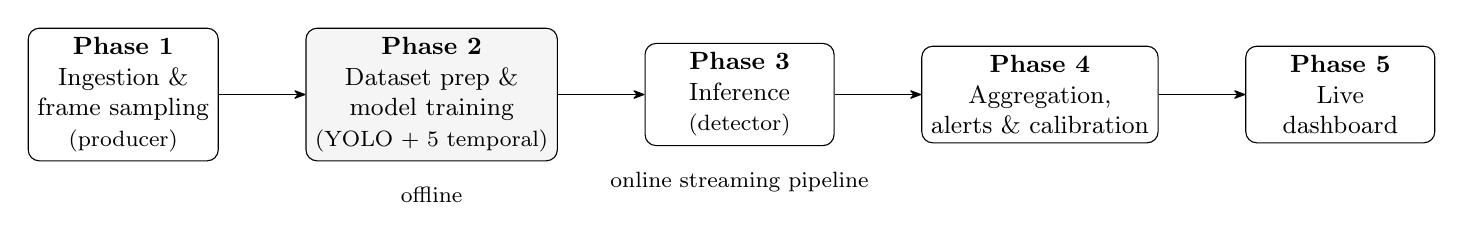
\begin{tikzpicture}[
    node distance=8mm and 11mm,
    box/.style={draw,rounded corners,align=center,minimum height=11mm,
                minimum width=24mm,font=\small},
    >={Stealth[round]}]
  \node[box] (ingest) {\textbf{Phase 1}\\Ingestion \&\\frame sampling\\
                       \footnotesize(producer)};
  \node[box,right=of ingest,fill=black!4] (train)
        {\textbf{Phase 2}\\Dataset prep \&\\model training\\
         \footnotesize(YOLO + 5 temporal)};
  \node[box,right=of train] (infer)
        {\textbf{Phase 3}\\Inference\\\footnotesize(detector)};
  \node[box,right=of infer] (agg)
        {\textbf{Phase 4}\\Aggregation,\\alerts \& calibration};
  \node[box,right=of agg] (dash)
        {\textbf{Phase 5}\\Live\\dashboard};

  \draw[->] (ingest) -- (train);
  \draw[->] (train)  -- (infer);
  \draw[->] (infer)  -- (agg);
  \draw[->] (agg)    -- (dash);

  \node[font=\footnotesize,below=2mm of train] (off) {offline};
  \node[font=\footnotesize,below=2mm of infer] {online streaming pipeline};
\end{tikzpicture}
\caption{The five methodology phases. Phase~2 (shaded) is the offline training
step; Phases~1 and 3--5 form the online streaming pipeline.}
\label{fig:methodology-phases}
\end{figure*}

\subsection{Architecture Overview}
\label{subsec:architecture}

The SafeStream-Kafka data flow is shown in
Fig.~\ref{fig:system-architecture}. The pipeline is structured as producer
$\rightarrow$ detector $\rightarrow$ aggregator $\rightarrow$ dashboard, with
the four services communicating only through three Kafka topics. In
Fig.~\ref{fig:system-architecture}, solid boxes are the four services, cylinders
are the Kafka topics that connect them, and dashed boxes are the external video
sources and the browser.

To keep one responsibility per service and a single source of truth for every
alert, we designate the \emph{standalone aggregator} as the sole authoritative
owner of alerting: it alone consumes \texttt{safety-detections}, evaluates the
sliding window, and publishes to \texttt{safety-alerts}. The dashboard is a
strictly \emph{read-only} consumer it subscribes to \texttt{safety-alerts} to
display alerts and to \texttt{cctv-frames} to show the latest camera images, runs
no aggregation logic of its own, and never writes to \texttt{safety-alerts}.

% The prototype does not yet enforce this separation. The dashboard
% currently embeds its own copy of the aggregator and republishes alerts in
% parallel with the standalone service. Because the two subscribe under
% \emph{different} Kafka consumer groups, each receives every detection
% independently rather than sharing the load, so running both at once makes both
% emit alerts for the same event producing duplicate alerts and divergent
% window state. This is a genuine race in alert ownership, not merely cosmetic
% redundancy. Consolidating onto the read-only dashboard described above removes
% it by construction; Section~\ref{sec:limitations} discusses completing that
% migration.

The runtime pipeline separates video ingestion, model inference, aggregation,
and dashboard visualization. The producer publishes encoded frames to
\texttt{cctv-frames}; the detector consumes those frames and publishes
safety-detection summaries to \texttt{safety-detections}; the standalone
aggregator maintains per-camera rolling state and alert logic; and the dashboard
consumes stream outputs to display live camera images, rolling ratios, recent
alerts, unsafe-behavior summaries, and operational metrics.

This separation keeps the pipeline modular while still supporting the live
dashboard shown in the prototype. Kafka topics provide the contract between
services, so each component can be developed, tested, and scaled independently.


\begin{figure*}[t]
\centering
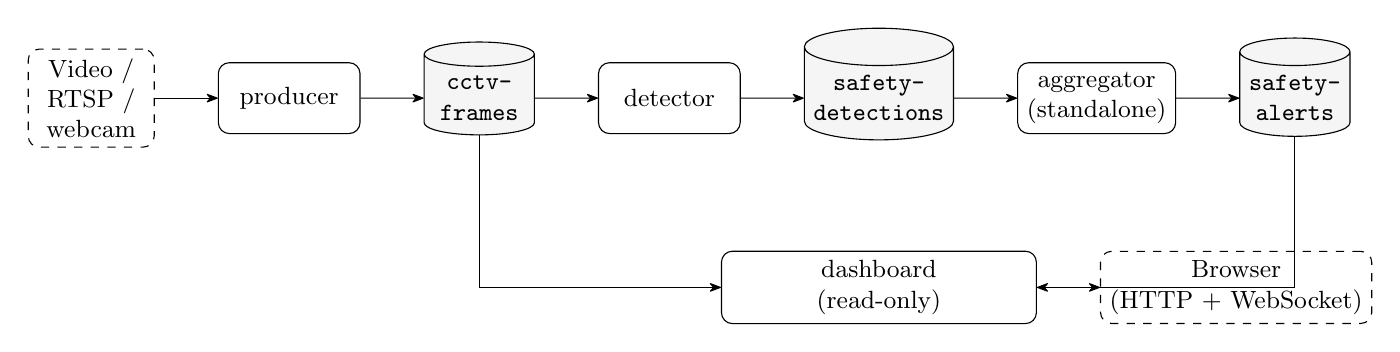
\begin{tikzpicture}[font=\small,>={Stealth[round]},
    node distance=6mm and 8mm,
    svc/.style={draw,rounded corners,minimum height=9mm,minimum width=18mm,
                align=center},
    topic/.style={draw,cylinder,shape border rotate=90,aspect=0.25,
                  fill=black!4,minimum height=11mm,minimum width=14mm,
                  align=center},
    ext/.style={draw,dashed,rounded corners,minimum height=9mm,
                minimum width=16mm,align=center}]
  \node[ext] (src) {Video /\\RTSP /\\webcam};
  \node[svc,right=of src] (prod) {producer};
  \node[topic,right=of prod] (frames) {\texttt{cctv-}\\\texttt{frames}};
  \node[svc,right=of frames] (det) {detector};
  \node[topic,right=of det] (dets) {\texttt{safety-}\\\texttt{detections}};
  \node[svc,right=of dets] (agg) {aggregator\\(standalone)};
  \node[topic,right=of agg] (alerts) {\texttt{safety-}\\\texttt{alerts}};

  \draw[->] (src)    -- (prod);
  \draw[->] (prod)   -- (frames);
  \draw[->] (frames) -- (det);
  \draw[->] (det)    -- (dets);
  \draw[->] (dets)   -- (agg);
  \draw[->] (agg)    -- (alerts);

  \node[svc,below=14mm of dets,minimum width=40mm] (dash)
        {dashboard\\(read-only)};
  \node[ext,right=of dash] (browser) {Browser\\(HTTP + WebSocket)};

  \draw[->] (frames) |- (dash);
  \draw[->] (alerts) |- (dash);
  \draw[->] (dash)   -- (browser);
\end{tikzpicture}
\caption{SafeStream-Kafka runtime architecture in the resolved single-owner
design: the standalone aggregator is the only producer of \texttt{safety-alerts},
and the dashboard is a read only consumer of \texttt{safety-alerts} (for alerts)
and \texttt{cctv-frames} (for live images).}
\label{fig:system-architecture}
\end{figure*}


\subsection{Data Model and Kafka Topics}

The producer sends one message for each selected frame. Each message carries a
camera identifier (also used as the Kafka message key, so each camera maps to one
ordered partition), a frame number that increases over time, the source (a video
path, RTSP URL, or webcam), a timestamp recorded when the frame is published, and
the frame image itself, stored as a JPEG encoded into text so it can travel
inside the message.

The detector consumes those frame messages and publishes detection summaries.
A classification model produces a single best guess label and a confidence score
for the frame. A detection model produces labels, confidence scores, and bounding
boxes for predicted regions.

The safety mapping is deliberately simple and easy to inspect: behaviors such as
an opened panel cover, an unauthorized intervention, or carrying an overload with
a forklift are treated as unsafe, while an authorized intervention, a closed
panel cover, or wearing a safety vest are treated as safe.

\subsection{Producer Methodology}
The producer accepts one or more video files, a directory of clips or, an RTSP stream, samples frames at a configurable analytics FPS, JPEG encodes the selected frames, and publishes them to Kafka with the camera ID as the key, preserving per camera order when Kafka partitions by key.

\subsection{Detector Methodology}

The detector loads YOLO weights from a configurable path and runs on an
Apple-silicon GPU, an NVIDIA GPU, or the CPU, whichever is available. For each
\texttt{cctv-frames} message, it decodes the JPEG frame, runs inference, and
writes the result to \texttt{safety-detections}.

It handles two output formats:

\begin{itemize}
    \item \textbf{Classification mode:} takes the model's per-frame class
    probabilities, uses the most likely class and its confidence, and emits one
    label per frame when the confidence exceeds the configured threshold.

    \item \textbf{Detection mode:} takes the model's predicted bounding boxes,
    iterates over them, and emits labels, confidence scores, and bounding-box
    coordinates.
\end{itemize}

Keeping both modes avoids locking the project to one dataset format.
The available dataset supports classification. A later bounding-box
dataset could use the same streaming pipeline for localized violations.

\subsection{Aggregation and Alert Methodology}
\label{subsec:aggregation}

The aggregator processes incoming detection summaries sequentially to maintain independent state engines for each camera stream. Each message contributes to both a continuous time-series smoothing pipeline and a categorical rolling window. This dual track architecture converts individual frame inferences into stable, operational metrics using two distinct alerting mechanisms: the \textit{Rolling-Ratio Rule} and the \textit{Smoothed-Probability Rule}.

\begin{figure*}[t]
\centering
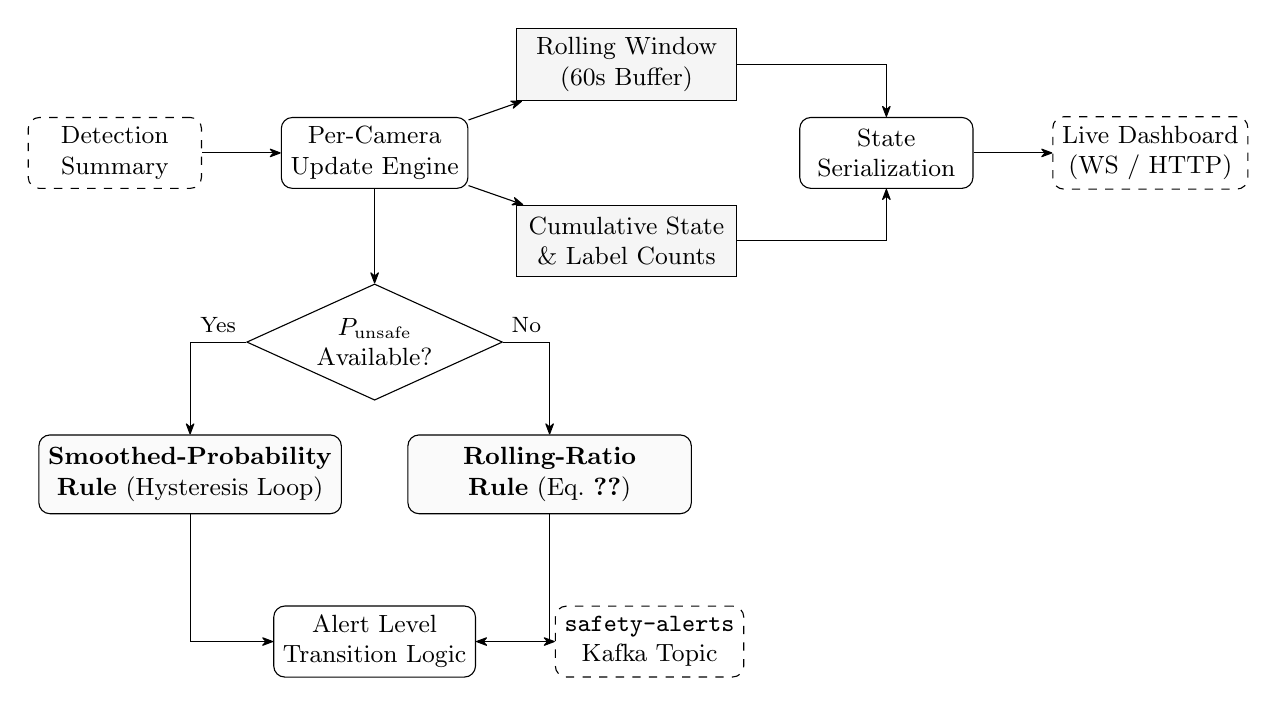
\begin{tikzpicture}[font=\small, >={Stealth[round]},
    node distance=5mm and 10mm,
    io/.style={draw, dashed, rounded corners, align=center, minimum height=9mm, minimum width=22mm},
    proc/.style={draw, rounded corners, align=center, minimum height=9mm, minimum width=22mm},
    state/.style={draw, fill=black!4, align=center, minimum height=9mm, minimum width=28mm},
    dec/.style={draw, diamond, aspect=2.2, align=center, inner sep=2pt},
    rule/.style={draw, rounded corners, align=center, fill=black!2, minimum height=10mm, minimum width=36mm}]

  % --- Top Tier: Ingest -> State -> Dashboard ---
  \node[io] (in) {Detection\\Summary};
  \node[proc, right=of in] (upd) {Per-Camera\\Update Engine};
  \node[state, above right=2mm and 6mm of upd] (win) {Rolling Window\\(60s Buffer)};
  \node[state, below right=2mm and 6mm of upd] (tot) {Cumulative State\\\& Label Counts};
  \node[proc, right=4.2cm of upd] (snap) {State\\Serialization};
  \node[io, right=of snap] (dash) {Live Dashboard\\(WS / HTTP)};

  \draw[->] (in) -- (upd);
  \draw[->] (upd) -- (win);
  \draw[->] (upd) -- (tot);
  \draw[->] (win) -| (snap);
  \draw[->] (tot) -| (snap);
  \draw[->] (snap) -- (dash);

  % --- Bottom Tier: Dual-Rule Alert Engine ---
  \node[dec, below=1.2cm of upd] (dec) {$P_{\text{unsafe}}$\\Available?};
  \node[rule, below left=8mm and -4mm of dec] (r2) {\textbf{Smoothed-Probability}\\\textbf{Rule} (Hysteresis Loop)};
  \node[rule, below right=8mm and -4mm of dec] (r1) {\textbf{Rolling-Ratio}\\\textbf{Rule} (Eq.~\ref{eq:rolling-unsafe-ratio})};
  \node[proc, below=2.6cm of dec] (alert) {Alert Level\\Transition Logic};
  \node[io, right=of alert] (out) {\texttt{safety-alerts}\\Kafka Topic};

  \draw[->] (upd) -- (dec);
  \draw[->] (dec) -| (r2) node[near start, above, font=\footnotesize] {Yes};
  \draw[->] (dec) -| (r1) node[near start, above, font=\footnotesize] {No};
  \draw[->] (r2) |- (alert);
  \draw[->] (r1) |- (alert);
  \draw[->] (alert) -- (out);
\end{tikzpicture}
\caption{The dual track aggregator architecture. The top tier handles real time state mutations for dashboard visualization, while the bottom tier orchestrates the conditional alerting logic.}
\label{fig:aggregator}
\end{figure*}

\subsubsection{Rolling-Ratio Rule}
The first mechanism evaluates categorical behavior classifications within a sliding temporal window of duration $W$ (defaulting to 60 seconds). For each camera, let $N_{\mathrm{rolling\_safe}}$ and $N_{\mathrm{rolling\_unsafe}}$ denote the respective counts of safe and unsafe frame labels within the active window. The rolling unsafe ratio, $R_{\mathrm{unsafe}}$, is calculated dynamically as:

\begin{equation}
R_{\mathrm{unsafe}} = \frac{N_{\mathrm{rolling\_unsafe}}}{N_{\mathrm{rolling\_safe}} + N_{\mathrm{rolling\_unsafe}}}
\label{eq:rolling-unsafe-ratio}
\end{equation}

The system transitions between discrete system \textit{Alert Levels} by comparing $R_{\mathrm{unsafe}}$ against predefined statistical thresholds, provided a minimum observation count ($N \ge 5$) is met to prevent transient initialization spikes. The default operational thresholds are structured as follows:
\begin{itemize}
    \item \textbf{Safe State:} $R_{\mathrm{unsafe}} < 0.30$
    \item \textbf{Warning Alert:} $0.30 \le R_{\mathrm{unsafe}} < 0.60$
    \item \textbf{High Severity Alert:} $R_{\mathrm{unsafe}} \ge 0.60$
\end{itemize}

\subsubsection{Smoothed-Probability Rule}
The second mechanism bypasses hard categorical assignments, operating instead on the raw continuous \textit{unsafe probability} scores emitted directly by the deep learning backbones. Let $P_t \in [0, 1]$ represent the raw unsafe probability generated by the model at frame event $t$. To insulate the downstream monitoring logic from high-frequency inference noise and single-frame anomalies, the aggregator computes a smoothed unsafe probability, $S_t$, using an Exponentially Weighted Moving Average (EWMA):

\begin{equation}
S_t = \alpha P_t + (1 - \alpha)S_{t-1}
\label{eq:ewma}
\end{equation}
where $\alpha \in (0, 1]$ is the smoothing factor configuring the system's temporal sensitivity. 

To govern alert generation without causing rapid state-flapping, this rule implements a hysteresis loop utilizing two model-specific decision thresholds: an activation threshold ($\tau_{\text{start}}$) and a deactivation threshold ($\tau_{\text{end}}$), where $\tau_{\text{start}} > \tau_{\text{end}}$. 

An alert event is instantiated when $S_t \ge \tau_{\text{start}}$ persists for a minimum consecutive frame sequence, collapsing an entire unsafe episode into a single persistent alert track. The alert remains active until the smoothed probability falls below the lower threshold ($S_t < \tau_{\text{end}}$). 

Crucially, because distinct model architectures scale their internal logit distributions differently, the activation threshold $\tau_{\text{start}}$ cannot be a fixed global constant. Instead, the alert level activation must be explicitly calibrated per model on an independent validation split to align the trigger points with an identical target recall rate, as detailed in Section~\ref{subsec:streaming-alerts}.

\subsection{Dashboard Methodology}

The FastAPI dashboard runs background Kafka consumers for detection
summaries and recent frame payloads. It makes the following available to the
browser:

\begin{itemize}
    \item current per-camera totals and rolling ratios;

    \item recent alert history;

    \item recent aggregation history;

    \item a recent frame for a given camera, with detection overlays drawn when
    bounding boxes are available;

    \item the last annotated violation frame for a given camera, when one exists;

    \item a live update channel that refreshes the dashboard about once a second.
\end{itemize}

For a classroom demonstration, the dashboard shows per camera safe and
unsafe counts, rolling unsafe ratios, recent alerts, live frame freshness,
and violation information.



\subsection{Dataset and Training Methodology}

The project targets the Voxel51 Safe and Unsafe Behaviours dataset~\cite{b6}.
Because the dataset has
clip level labels rather than bounding boxes, a dataset preparation step builds
a YOLO classification folder tree by sampling evenly spaced frames from each
clip. This avoids the earlier weak approximation of using whole frame boxes for
a detection model.

The training step then trains a YOLO image classifier, starting from an
ImageNet-pretrained classification model, with a default image size of 224 and
automatic device selection. All model training, offline evaluation, and
live streaming measurements reported in this paper were carried out on a single
workstation equipped with an NVIDIA GeForce RTX 3060 Ti GPU (8\,GB). The main
dataset-preparation and training settings are summarized in
Table~\ref{tab:dataset-config}.

\begin{table}[!t]
\centering
\caption{Dataset Preparation and YOLO Classifier Training Configuration}
\label{tab:dataset-config}
\renewcommand{\arraystretch}{1.08}
\setlength{\tabcolsep}{3.5pt}

\begin{tabularx}{\columnwidth}{
    >{\raggedright\arraybackslash}p{2.25cm}
    >{\raggedright\arraybackslash}X
}
\toprule
\textbf{Item} & \textbf{Configuration} \\
\midrule

Dataset source &
Voxel51 Safe and Unsafe Behaviours \\

Annotation type &
Clip level behavior labels; no bounding-box annotations \\

Learning task &
YOLOv8 image classification \\

Frame extraction &
Up to 12 evenly spaced frames per video clip \\

Hub split &
70\% training, 20\% validation, and 10\% testing \\

Random seed &
42 \\

Output structure &
One folder per split (train, validation, test), each with one subfolder per
class \\

Starting model &
ImageNet-pretrained YOLOv8 classification model (medium) \\

Image size &
224 $\times$ 224 pixels \\

Training epochs &
50 \\

Batch size &
16 \\

Training hardware &
NVIDIA GeForce RTX 3060 Ti GPU (8\,GB); code auto selects an Apple silicon GPU,
an NVIDIA GPU, or the CPU \\

\bottomrule
\end{tabularx}
\end{table}

\subsubsection{Temporal Window Models}

The per-frame YOLO classifier is one of the two model families trained for
this project. To test whether motion across frames helps
(Section~\ref{subsec:research-questions}, RQ2), Phase~2 also trains five
\emph{temporal window models} that classify a short clip from a stack of
frames. These models do not use the YOLO classification tree; instead a separate
training step reads a clip manifest a table listing each clip's file path,
label, and train/val/test split and decodes a fixed window of frames per clip
with the same evenly spaced selection used by the per frame pipeline. Decoded
and resized frames are cached on disk, keyed by image size and frame
count, so repeated runs and all 224 pixel models reuse one cache.

A single model factory constructs every
kind, so the same training, evaluation, and live-inference code
serves all of them. The five kinds are an in house ResNet18+GRU
head~\cite{b11,b12}, a torchvision R(2+1)D-18~\cite{b7}, and three
Kinetics-400-pretrained~\cite{b13} video transformers
(MViTv2-S~\cite{b8}, Video Swin-T~\cite{b9}, and Hiera-B~\cite{b10}).
The three transformers
are \emph{linear-probed}: the pretrained backbone is frozen and only a
fresh, roughly six thousand parameter head is trained, which keeps them
within an 8\,GB GPU. The optimizer filters to trainable parameters, so a
frozen backbone trains only its head automatically. MViTv2-S and Hiera-B
have fixed positional embeddings and require a 16 frame window, so all
window models use 16 frames for a fair comparison.

Training and evaluation were handled by a shared ablation runner so that all
temporal models used matched conditions. The temporal models used 16-frame
windows, 224$\times$224 inputs, RTX 3060 Ti hardware, and linear probing for the
transformer backbones. The alert threshold was calibrated per model on the
validation split because each model placed its unsafe probability on a different
scale.

% Training and both evaluation stages are orchestrated by a single ablation
% runner, which trains every kind under identical
% conditions and then measures offline accuracy, streaming alert quality,
% parameter count, and per-frame latency. Crucially, because each model
% places its unsafe probability on a different scale, the streaming alert
% threshold is \emph{calibrated per model} on the validation split (sweeping
% the aggregator's start and clear levels to a recall target before reporting on
% the test split), as discussed in Section~\ref{subsec:aggregation}. The
% shared temporal-training settings are summarized in
% Table~\ref{tab:temporal-config}.

% \begin{table}[!t]
% \centering
% \caption{Temporal Window-Model Training and Ablation Configuration}
% \label{tab:temporal-config}
% \renewcommand{\arraystretch}{1.08}
% \setlength{\tabcolsep}{3.5pt}

% \begin{tabularx}{\columnwidth}{
%     >{\raggedright\arraybackslash}p{2.25cm}
%     >{\raggedright\arraybackslash}X
% }
% \toprule
% \textbf{Item} & \textbf{Configuration} \\
% \midrule

% Models &
% ResNet18+GRU head, R(2+1)D-18, MViTv2-S, Video Swin-T, Hiera-B \\

% Window length &
% 16 frames per clip \\

% Frame sampling &
% Evenly spaced selection matching the per-frame pipeline; decoded frames
% cached by image size and count \\

% Pretraining &
% ImageNet (head backbone); Kinetics-400 (R(2+1)D-18 and the three
% transformers) \\

% Transformer training &
% Linear probe; frozen backbone, fresh approximately 6K-parameter head \\

% Optimizer &
% AdamW over the trainable parameters (the frozen backbone is skipped
% automatically) \\

% Image size &
% 224 $\times$ 224 pixels \\

% Alert threshold &
% Calibrated per model on the validation split (recall target, lowest
% false-alert rate) \\

% Orchestration &
% A single ablation runner trains and evaluates all kinds under identical
% conditions \\

% Training hardware &
% NVIDIA GeForce RTX 3060 Ti GPU (8\,GB) \\

% \bottomrule
% \end{tabularx}
% \end{table}



% =========================================================
% 4. Data Analytics and Results
% =========================================================
\section{Data Analytics and Results}

% 4.1 Evaluation Scope
\subsection{Evaluation Scope}

This section reports measured results both \emph{offline} (on the fixed
test split) and \emph{streaming} (from the running pipeline) for the
shipped per frame classifier and a six model comparison. The per frame offline
metrics are computed on 1500 sampled test frames, and every number in this
section traces to a saved results file. End to end latency, throughput,
frame transport overhead, and consumer lag are measured on the running pipeline
in Section~\ref{subsec:systems}; GPU and memory utilization under load and
large-scale multi-camera scaling remain future work
(Section~\ref{sec:limitations}).

% 4.2 Offline Classification Results
\subsection{Offline Classification Results}

Table~\ref{tab:offline-metrics} reports the per frame classifier on the
test split. Precision is the share of frames flagged unsafe that were
unsafe; recall is the share of unsafe frames that were flagged. Average
precision is the area under the precision --- recall curve. The 8 class
accuracy is the share of frames whose predicted behavior matched
the labeled behavior across the eight behavior classes; the 8 class macro
average precision averages the per class average precision. These are
classification metrics, not bounding-box overlap.

\begin{table}[!t]
\centering
\caption{Per-frame classifier on the test split.}
\label{tab:offline-metrics}
\renewcommand{\arraystretch}{1.15}
\begin{tabularx}{\columnwidth}{
    >{\raggedright\arraybackslash}X
    >{\raggedleft\arraybackslash}p{2.0cm}
}
\toprule
\textbf{Metric} & \textbf{Value} \\
\midrule
Binary unsafe precision & 0.769 \\
Binary unsafe recall & 0.841 \\
Binary unsafe F1 & 0.803 \\
Binary unsafe average precision & 0.887 \\
Safe-vs-unsafe accuracy & 0.789 \\
8-class accuracy & 0.641 \\
8-class macro average precision & 0.729 \\
\midrule
True positives (unsafe) & 646 \\
False positives & 194 \\
False negatives & 122 \\
True negatives & 538 \\
\bottomrule
\end{tabularx}
\end{table}

% 4.3 Model Comparison
\subsection{Model Comparison}

Table~\ref{tab:model-comparison} compares the per frame classifier with
five window models on the same data. The five window models are an
in-house ResNet18+GRU head~\cite{b11,b12}, a torchvision
R(2+1)D-18~\cite{b7}, and three Kinetics-400-pretrained~\cite{b13} video
transformers: MViTv2-S~\cite{b8} and Video Swin-T~\cite{b9} from
torchvision, and Hiera-B~\cite{b10} from a public Hiera implementation.
The three transformers kept their main layers fixed and trained only a
small final layer, and all window models use a 16 frame window. In the
table, the offline columns are over the test split: unsafe AP is the
average precision for the unsafe class, F1 balances unsafe precision and
recall, and 8 class accuracy is the share of frames whose predicted
behavior matched the label across the eight classes. The streaming
columns use a per-model alert start level chosen on the validation set
(Section~\ref{subsec:streaming-alerts}): ``safe clips alerted'' is the
share of safe clips that produced at least one alert, and Alert P and
Alert R are the alert precision and recall. Time per frame was measured on
the workstation's NVIDIA GeForce RTX 3060 Ti (8\,GB) GPU.

\begin{table*}[t]
\centering
\caption{Six-model comparison.}
\label{tab:model-comparison}
\renewcommand{\arraystretch}{1.25}
\begin{tabularx}{\textwidth}{
    >{\raggedright\arraybackslash}p{3.0cm}
    >{\raggedleft\arraybackslash}X
    >{\raggedleft\arraybackslash}X
    >{\raggedleft\arraybackslash}X
    >{\raggedleft\arraybackslash}X
    >{\raggedleft\arraybackslash}X
    >{\raggedleft\arraybackslash}X
    >{\raggedleft\arraybackslash}X
}
\toprule
\textbf{Model} &
\textbf{Offline unsafe AP} &
\textbf{F1} &
\textbf{8-class accuracy} &
\textbf{Safe clips alerted} &
\textbf{Alert P} &
\textbf{Alert R} &
\textbf{Time/frame (ms)} \\
\midrule
YOLOv8 (per-frame) & 0.887 & 0.803 & 0.641 & 0.311 & 0.732 & 0.812 & 6.40 \\
head (ResNet18+GRU) & 0.862 & 0.704 & 0.440 & 0.557 & 0.634 & 0.922 & 13.63 \\
video (R(2+1)D-18) & 0.755 & 0.695 & 0.472 & 0.705 & 0.578 & 0.922 & 26.39 \\
MViTv2-S & 0.795 & 0.707 & 0.488 & 0.852 & 0.544 & 0.969 & 48.38 \\
Video Swin-T & 0.805 & 0.702 & 0.480 & 0.623 & 0.596 & 0.875 & 39.76 \\
Hiera-B & 0.862 & 0.727 & 0.536 & 0.787 & 0.571 & 1.000 & 46.96 \\
\bottomrule
\end{tabularx}
\end{table*}

% 4.4 Streaming Alerts and Alert-Level Setting
\subsection{Streaming Alerts and Alert-Level Setting}
\label{subsec:streaming-alerts}

In the stream, the per frame classifier produced alert precision 0.732
and alert recall 0.812, and 0.311 of safe clips produced an alert. It
used 6.40 ms per frame. These streaming numbers are over 125 test clips
(64 unsafe and 61 safe); the offline metrics in
Table~\ref{tab:offline-metrics} are over 1500 frames.

The alert start level had to be chosen with care. With one fixed start
level, most models alerted on nearly every clip, because each model puts
its unsafe probability on a different scale. Choosing the start level per
model on the validation split, using the smoothed probability rule in
Section~\ref{subsec:aggregation}, removed this: the chosen start levels
ranged from 0.45 to 0.70 across the six models, and the per frame
classifier settled at 0.60 with the 0.311 share of safe clips alerted
reported above.

% 4.5 Findings
\subsection{Findings}
\label{subsec:findings}

The six-model comparison answers the three research questions posed in
Section~\ref{subsec:research-questions}:
\begin{itemize}
\item \textbf{(RQ2)} The per-frame YOLO classifier achieved the best offline
result, with 0.887 unsafe AP and 0.641 8 class accuracy; temporal window models
did not improve accuracy on this dataset, likely because many unsafe behaviours
are visible in a single frame. They did not improve alert quality either: the
per-frame classifier produced the fewest false alerts (0.311 of safe clips
alerted) at the lowest cost (6.40\,ms per frame), so the window models' extra
per-frame cost was not justified here.
\item \textbf{(RQ1)} Offline accuracy did not always predict streaming
false alert behaviour, so the two must be measured separately --- two models with
the same 0.862 offline unsafe AP alerted on 0.557 (head) and 0.787 (Hiera-B) of
safe clips.
\item \textbf{(RQ3)} A single fixed alert level did not serve every model:
thresholds needed per model calibration because each model produced unsafe
probabilities on a different scale, with chosen start levels ranging from 0.45
to 0.70.
\end{itemize}

These results should be read within this dataset and compute budget: several
transformer backbones were linear probed rather than fully fine tuned, and the
main unsafe behaviours were often visible in a single frame.
Section~\ref{subsec:systems} complements these model-quality findings with
systems-level measurements.

% The comparison gives five findings, which together answer the three
% research questions posed in Section~\ref{subsec:research-questions}
% (RQ1--RQ3):

% \begin{itemize}
%     \item \textbf{(RQ2)} The per-frame classifier had the highest offline
%     accuracy of the six models (8-class accuracy 0.641 versus 0.440--0.536;
%     binary unsafe average precision 0.887 versus 0.755--0.862).

%     \item \textbf{(RQ2)} Using a 16-frame window did not raise accuracy on
%     this dataset; the likely reason is that the unsafe behaviors in this
%     dataset can be seen in a single frame, although we do not measure this
%     directly.

%     \item \textbf{(RQ1)} A model's offline accuracy did not reliably rank
%     the models by how many false alerts they produced. The best offline
%     model (the per-frame classifier) was also the best in the stream, but
%     among the remaining models the ranking broke down: two models with the
%     same offline average precision (0.862) had shares of safe clips alerted
%     of 0.557 (head) and 0.787 (Hiera-B). Offline accuracy therefore carries
%     some signal but cannot stand in for a streaming measurement.

%     \item \textbf{(RQ3)} The alert start level has to be set per model; the
%     chosen levels ranged from 0.45 to 0.70.

%     \item \textbf{(RQ2)} The per-frame classifier produced the fewest false
%     alerts (0.311 of safe clips) and used the least time per frame
%     (6.40 ms).
% \end{itemize}

% The RQ2 result deserves a methodological caveat. The three transformers
% (MViTv2-S, Video Swin-T, and Hiera-B) were deliberately resource-constrained: to
% stay within the RTX 3060 Ti's 8\,GB they were \emph{linear-probed}, freezing their
% Kinetics-400 backbones and training only a fresh ${\sim}6$K-parameter head.
% Freezing the spatio-temporal backbone limits how far each model can adapt to this
% workplace dataset, so their lower accuracy may reflect that constrained training
% regime rather than an inherent inability to exploit temporal context; full
% fine-tuning under a larger GPU budget could narrow the gap and is left to future
% work. Two observations temper this reading, however. First, the R(2+1)D-18 model
% was \emph{fully} fine-tuned---all 31\,M parameters trainable---and still trailed
% the per-frame classifier on both offline accuracy and streaming false-alert rate,
% so the single-frame advantage is not purely an artifact of frozen backbones.
% Second, the unsafe behaviors in this dataset are visible within a single frame,
% which bounds how much temporal modeling can add. We therefore read RQ2 narrowly:
% on \emph{this} single-frame-visible task and under \emph{this} compute budget, the
% window models did not justify their extra per-frame cost---not as a general claim
% that temporal models cannot help.

% These findings carry five caveats. The offline metrics are over 1500
% frames for the per-frame model but over 125 clips for the window models.
% The per-frame model's lower share of safe clips alerted comes with a
% lower test recall (alert recall 0.812 versus 0.875--1.000 for the window
% models). The time-per-frame numbers were measured on the workstation's
% NVIDIA GeForce RTX 3060 Ti (8\,GB) GPU. The labeled set covers behaviors that
% are visible in a single
% frame. Finally, the three transformer models were linear-probed under the
% RTX 3060 Ti's 8\,GB budget, so their reported accuracy is a lower bound on what full
% fine-tuning might achieve.

% Section~\ref{subsec:systems} complements these model-quality findings with
% systems-level measurements---end-to-end latency, throughput, frame-transport
% overhead, and consumer lag---taken on the running pipeline.

% 4.x Systems-Level Performance
\subsection{Systems-Level Performance}
\label{subsec:systems}

The metrics above measure alert quality; this subsection summarizes the
streaming system measurements. In the controlled live run, the per frame YOLO
classifier ran against a Confluent Cloud broker with frames sampled at the
default analytics rate of 4\,fps. The pipeline achieved a mean end to end
latency of 0.198\,s, a maximum latency of 0.379\,s, and sustained throughput of
3.98\,fps with zero consumer lag. Each base64 JSON frame cost about 352\,KB on
the wire, or about 1.38\,MB/s per camera at 4\,fps. Based on the measured
inference time of 6.40\,ms per frame, the YOLOv8 per frame classifier has a
single-stream throughput ceiling of about 156\,fps. These results show that the
GPU was not the bottleneck at the classroom analytics rate, while Kafka buffering
allowed temporary bursts to accumulate and drain without dropped records.

% The metrics above measure alert quality; this subsection measures the streaming
% \emph{system}. Unless stated otherwise, numbers were collected with the per-frame
% YOLO classifier running live against a Confluent Cloud broker (SASL\_SSL) on the
% evaluation machine (NVIDIA GeForce RTX 3060 Ti, 8\,GB), with frames sampled at the default analytics
% rate of 4\,fps. Two measurements support this subsection---an offline sizing of
% the frame payload and a probe of Kafka consumer-group lag---and both are
% reproducible from the source repository~\cite{b14}.

% \subsubsection{Frame-transport overhead}
% Each frame travels as a JPEG that is base64-encoded inside a JSON message so it
% can ride within a Kafka record. Table~\ref{tab:payload} traces that cost over 192
% sampled 1080p demo frames. JPEG removes most of the raw cost---a frame shrinks to
% 4.3\% of its uncompressed size---but base64 then re-inflates the image by exactly
% one third (a 4:3 expansion), and the broker's configured \texttt{lz4} compression
% recovers essentially none of it because a JPEG is already entropy-coded. Net, a
% frame costs about 352\,KB on the wire versus 264\,KB as a raw JPEG, or roughly
% 1.4\,MB/s per camera at 4\,fps. A binary frame topic would remove the 33\% base64
% tax; we keep the text encoding for its inspectability in this prototype.

% \begin{table}[!t]
% \centering
% \caption{Per-frame transport cost (mean over 192 sampled 1080p frames, JPEG
% quality 80).}
% \label{tab:payload}
% \renewcommand{\arraystretch}{1.15}
% \setlength{\tabcolsep}{3.5pt}
% \begin{tabularx}{\columnwidth}{
%     >{\raggedright\arraybackslash}X
%     >{\raggedleft\arraybackslash}p{1.7cm}
%     >{\raggedleft\arraybackslash}p{1.7cm}
% }
% \toprule
% \textbf{Representation} & \textbf{Mean size} & \textbf{vs.\ JPEG} \\
% \midrule
% Raw BGR frame (1920$\times$1080) & 6075 KB & 23.0$\times$ \\
% JPEG (quality 80) & 264 KB & 1.00$\times$ \\
% Base64 text & 352 KB & 1.33$\times$ \\
% Full JSON message & 352 KB & 1.33$\times$ \\
% lz4-compressed (on wire) & 352 KB & 1.33$\times$ \\
% \midrule
% Per camera at 4\,fps & \multicolumn{2}{r}{$\approx$\,1.38 MB/s} \\
% \bottomrule
% \end{tabularx}
% \end{table}

% \subsubsection{End-to-end latency and throughput}
% With the producer publishing at 4\,fps, the dashboard observed a mean end-to-end
% latency of 0.198\,s and a maximum of 0.379\,s. Here ``end to end'' spans the
% producer's publish timestamp, the \texttt{cctv-frames} hop to the cloud broker,
% the detector's consume--infer--publish, the \texttt{safety-detections} hop back,
% and the dashboard's ingest; the dashboard's WebSocket then refreshes the browser
% at about 1\,Hz, adding up to a further ${\sim}1$\,s of on-screen latency.
% Sustained throughput matched the input at 3.98\,fps with the detector holding
% zero consumer lag, so the two cloud round-trips---not the GPU---dominate the
% figure.

% Per-frame inference leaves wide headroom over this 4\,fps operating point.
% Table~\ref{tab:throughput} converts each model's measured time per frame into a
% single-stream throughput ceiling: the per-frame classifier sustains about
% 156\,fps---an order of magnitude above the fastest window model and far above the
% analytics rate---while the video transformers fall to 21--25\,fps. The per-frame
% classifier is therefore not only the most accurate model here but also the one
% with the most streaming headroom.

% \begin{table}[!t]
% \centering
% \caption{Single-stream throughput ceiling derived from each model's measured time
% per frame (Table~\ref{tab:model-comparison}).}
% \label{tab:throughput}
% \renewcommand{\arraystretch}{1.15}
% \setlength{\tabcolsep}{3.5pt}
% \begin{tabularx}{\columnwidth}{
%     >{\raggedright\arraybackslash}X
%     >{\raggedleft\arraybackslash}p{2.0cm}
%     >{\raggedleft\arraybackslash}p{1.6cm}
% }
% \toprule
% \textbf{Model} & \textbf{Time/frame (ms)} & \textbf{Max FPS} \\
% \midrule
% YOLOv8 (per-frame) & 6.40 & 156 \\
% head (ResNet18+GRU) & 13.63 & 73 \\
% video (R(2+1)D-18) & 26.39 & 38 \\
% Video Swin-T & 39.76 & 25 \\
% Hiera-B & 46.96 & 21 \\
% MViTv2-S & 48.38 & 21 \\
% \bottomrule
% \end{tabularx}
% \end{table}

% \subsubsection{Backpressure and consumer lag}
% Decoupling ingestion from inference through Kafka is what lets the pipeline absorb
% a frame-rate spike without stalling the producer: unprocessed frames accumulate in
% \texttt{cctv-frames}---bounded only by topic retention---and the detector drains
% them once it catches up. We observed both directions of this. At the 4\,fps
% operating point the detector and dashboard consumer groups held zero lag; after we
% injected a burst of frames far above the 4\,fps rate, the detector group absorbed
% the backlog and returned to zero lag once the burst ended, with no records dropped
% by the broker. The buffering is clearest from an \emph{idle} group: with the
% standalone aggregator stopped, its committed offset stayed fixed while the topic
% kept advancing, so its lag grew monotonically (159 then 719 records over the
% session)---precisely the backlog Kafka retains on a stalled consumer's behalf.
% Under a flat-out burst the first bottleneck was in fact the producer's upload of
% the fat base64 frames (${\sim}10$\,MB/s, ${\sim}30$\,fps), which reinforces the
% transport finding above.

% If a sustained spike exceeded one detector's 6.40\,ms (156\,fps) budget, the
% architecture absorbs it three ways without changing the message contracts. First,
% the producer already samples at a fixed analytics FPS far below the camera's
% native frame rate, so it never offers the raw rate downstream. Second, the
% detector is a Kafka consumer group, so adding detector instances load-balances the
% \texttt{cctv-frames} partitions across them; because frames are keyed by
% \texttt{camera\_id}, each camera's order is preserved within its partition. Third,
% a consumer can skip stale frames to trade completeness for freshness when latency
% matters more than covering every frame. This elasticity is exactly what a
% monolithic offline script cannot provide, and it is why the streaming
% decomposition---not only the choice of model---is part of this work's
% contribution.

% 4.4 Dashboard Demonstration
\subsection{Dashboard Demonstration}

Figure~\ref{fig:dashboard-live} shows the SafeStream-Kafka dashboard
during a multi camera replay. The dashboard shows live camera monitoring,
safety classifications, rolling unsafe ratio tracking, alert activity, and
operational metrics in one interface, end to end from video ingestion to
visualization.

\begin{figure*}[t]
\centering

\includegraphics[width=\textwidth]{dashboard1.png}
\caption{The SafeStream-Kafka dashboard during a multi-camera replay.}
\label{fig:dashboard-live}
\end{figure*}

% =========================================================
% 5. Technical Writing Quality and Reproducibility
% =========================================================
\section{Technical Writing and Reproducibility}

The complete source code, setup instructions, and configuration for
SafeStream-Kafka are available in the project repository linked in the title
footnote. To
reproduce the prototype, follow the README, which documents the dependencies,
the local Kafka broker through Docker Compose and the Confluent Cloud
configuration, and the scripts for topic creation, dataset preparation, model
training, and running the four services.


% =========================================================
% 6. Limitations, Challenges, and Future Improvements
% =========================================================
\section{Limitations, Challenges, and Future Improvements}
\label{sec:limitations}

\subsection{Limitations}

These results come from one dataset. The offline metrics for the
per frame model are over 1500 test frames, and the six model streaming
comparison is over 125 test clips, so behavior on other sites, camera
placements, or unseen behaviors is not measured.

The dataset has clip-level labels and no bounding boxes. The per-frame
classifier reports whether a frame is unsafe, but it does not locate the
behavior inside the frame. A detection model could mark the region, but
it needs bounding-box labels that this dataset does not provide.

The live F1 and confusion values shown for arbitrary camera streams are
demo only. The dashboard derives ground truth from the clip filename, so
those values are meaningful only for the labeled demo clips, not for
unlabeled cameras.

End-to-end latency, throughput, frame transport overhead, and consumer lag
are now measured (Section~\ref{subsec:systems}), but on a single machine and a
single live camera stream. GPU and memory utilization under load, and scaling to
many simultaneous cameras across multiple detector instances, are not yet
profiled.

A second limitation is the as-built overlap in alert ownership. As described in
Section~\ref{subsec:architecture}, the dashboard currently embeds its own
aggregator and republishes alerts in parallel with the standalone aggregator;
because the two run under different consumer groups, running both duplicates
alerts and lets their window state diverge. The resolved design makes the
standalone aggregator the sole alert producer and reduces the dashboard to a
read-only consumer of \texttt{safety-alerts}; completing that migration --- removing
the dashboard's embedded aggregator --- is the remaining engineering work.

\subsection{Future Improvements}

The next development steps are measurable:

\begin{itemize}
    \item Extend the systems benchmarking of Section~\ref{subsec:systems} with
    GPU and memory utilization under load and with multi-camera, multi-detector
    scaling.

    \item Package the live latency, throughput, and lag measurement into a
    one-command replay harness so those numbers regenerate automatically.

    \item Provide a small public smoke test video or generated test
    stream that can exercise the pipeline without using private
    workplace data.

    \item Provide a checksum or external mirror for the committed classifier
    weights so others can verify the download.

    \item Remove the dashboard's embedded aggregator so that the standalone
    aggregator is the sole producer of \texttt{safety-alerts} and the dashboard
    consumes only \texttt{safety-alerts} and \texttt{cctv-frames}
    (Section~\ref{subsec:architecture}).

    \item Add an integration test using local Kafka through Docker
    Compose for a minimal producer to detector to aggregator/dashboard
    pipeline.

    \item Improve privacy controls through techniques such as frame
    redaction, retention limits, or edge only inference for sensitive
    workplace video.
\end{itemize}


% =========================================================
% 7. Conclusion
% =========================================================
\section{Conclusion}

SafeStream-Kafka publishes video frames through Kafka, labels each frame
with a per frame YOLO safety classifier, aggregates safe and unsafe counts
over time, fires alerts through a rolling ratio rule and a
smoothed-probability rule, and shows the result on a live dashboard. The
services communicate only through three Kafka topics, so each stage runs
as a separate process. This covers the implementation side of the rubric:
real time event processing, modular services, a running prototype, and
documented deployment procedures.

Across the six models compared on this dataset, the per-frame classifier
had the highest offline accuracy (8-class accuracy 0.641; binary unsafe
average precision 0.887), produced the fewest false alerts in the stream
(0.311 of safe clips alerted), and used the least time per frame
(6.40 ms)---giving it the highest single-stream throughput ceiling
($\sim$156\,fps). On the running pipeline, end-to-end latency averaged
0.198\,s through a cloud broker, throughput tracked the 4\,fps input with zero
consumer lag, and each base64-encoded frame cost about 352\,KB on the wire. GPU
utilization under load and multi-camera scaling remain to be profiled.



\section*{Member Contributions}
% Add each team member's contribution here.
Vitor Raposo: Led the management of the project alongside Ahmed. Participated in discussions, iterated on model training, model testing, ablation studies and dashboard development. Helped in paper writing and presentation setup. Recorded the DEMO.

Livia Zhang: Drafted the initial final report, trained and uploaded the YOLO model weights, refactored the dashboard with real-time video streaming and sliding-window display, and wrote the Docker Compose setup.

Yujie Lin: Supported safe/unsafe classification evaluation and dashboard risk-display improvements, including metric alignment, confusion-matrix interpretation, and the Highest Risk Camera summary. Formatted the IEEE report, created the system architecture diagram and dataset configuration table, and participated in proposal and presentation preparation.


Quang Thong Phung: Implemented the Kafka streaming pipeline, aggregation and alerting logic, dashboard backend services, and dashboard analytics enhancements including Top Unsafe Behaviors and Unsafe Ratio Trend visualization. Assisted with system testing and report preparation.

Ahmed Seyam: Supported the group through topic selection, model choosing, project proposal, aggregator code and overall project development feedback.

\begin{thebibliography}{00}
% NOTE: b1 author corrected from "S. S. Gill et al." to "A. A. Ravindran" -- the cited title is MDPI IoT 4(4):21 (2023) by Ravindran. Verify before submission.
\bibitem{b1} A. A. Ravindran, "Internet-of-Things Edge Computing Systems for Streaming Video Analytics: Trails Behind and the Paths Ahead," IoT, vol. 4, no. 4, pp. 486--513, 2023. [Online]. Available: \url{https://doi.org/10.3390/iot4040021}
\bibitem{b2} W. Zhang et al., "Edge Video Analytics: A Survey on Applications, Systems and Enabling Techniques," arXiv:2211.15751, 2022. [Online]. Available: \url{https://arxiv.org/abs/2211.15751}
\bibitem{b3} J. Kreps, N. Narkhede, and J. Rao, "Kafka: A Distributed Messaging System for Log Processing," in Proc. NetDB, 2011.
\bibitem{b4} Ultralytics, "Image Classification," Ultralytics Documentation. [Online]. Available: \url{https://docs.ultralytics.com/tasks/classify}
\bibitem{b5} Ultralytics, "Object Detection," Ultralytics Documentation. [Online]. Available: \url{https://docs.ultralytics.com/tasks/detect}
\bibitem{b6} O. Onal and E. Dandil, "Video dataset for the detection of safe and unsafe behaviours in workplaces," Data in Brief, vol. 56, Art. no. 110791, 2024. [Online]. Available: \url{https://doi.org/10.1016/j.dib.2024.110791}
\bibitem{b7} D. Tran, H. Wang, L. Torresani, J. Ray, Y. LeCun, and M. Paluri, "A Closer Look at Spatiotemporal Convolutions for Action Recognition," in Proc. IEEE/CVF Conf. Computer Vision and Pattern Recognition (CVPR), 2018, pp. 6450--6459. [Online]. Available: \url{https://arxiv.org/abs/1711.11248}
\bibitem{b8} Y. Li, C.-Y. Wu, H. Fan, K. Mangalam, B. Xiong, J. Malik, and C. Feichtenhofer, "MViTv2: Improved Multiscale Vision Transformers for Classification and Detection," in Proc. IEEE/CVF Conf. Computer Vision and Pattern Recognition (CVPR), 2022, pp. 4804--4814. [Online]. Available: \url{https://arxiv.org/abs/2112.01526}
\bibitem{b9} Z. Liu, J. Ning, Y. Cao, Y. Wei, Z. Zhang, S. Lin, and H. Hu, "Video Swin Transformer," in Proc. IEEE/CVF Conf. Computer Vision and Pattern Recognition (CVPR), 2022, pp. 3202--3211. [Online]. Available: \url{https://arxiv.org/abs/2106.13230}
\bibitem{b10} C. Ryali et al., "Hiera: A Hierarchical Vision Transformer without the Bells-and-Whistles," in Proc. Int. Conf. Machine Learning (ICML), 2023, pp. 29441--29454. [Online]. Available: \url{https://arxiv.org/abs/2306.00989}
\bibitem{b11} K. He, X. Zhang, S. Ren, and J. Sun, "Deep Residual Learning for Image Recognition," in Proc. IEEE Conf. Computer Vision and Pattern Recognition (CVPR), 2016, pp. 770--778. [Online]. Available: \url{https://arxiv.org/abs/1512.03385}
\bibitem{b12} K. Cho, B. van Merrienboer, C. Gulcehre, D. Bahdanau, F. Bougares, H. Schwenk, and Y. Bengio, "Learning Phrase Representations using RNN Encoder-Decoder for Statistical Machine Translation," in Proc. Conf. Empirical Methods in Natural Language Processing (EMNLP), 2014, pp. 1724--1734. [Online]. Available: \url{https://arxiv.org/abs/1406.1078}
\bibitem{b13} W. Kay et al., "The Kinetics Human Action Video Dataset," arXiv:1705.06950, 2017. [Online]. Available: \url{https://arxiv.org/abs/1705.06950}
% =========================================================

% \bibitem{b14} V. B. Raposo, Y. Lin, L. Zhang, Q. T. Phung, and A. Seyam, ``SafeStream-Kafka: source code,'' 2026. [Online]. Available: \url{https://github.com/Lumysia/SafeKafka}
% =========================================================

\end{thebibliography}

\end{document}
